\documentclass{beamer}
\usepackage[latin1]{inputenc}
\usepackage{multirow}
\usetheme{Goettingen} %Warsaw
\usecolortheme{seagull}


\title[Introduction to Sequencing]{Introduction to Sequencing}
\subtitle{BCB 511: Applied Bioinformatics\\}
\author[Matt Settles]{Matt Settles}
\institute{University of Idaho}
\date{\today}


\begin{document}



%% Title page
\begin{frame}[plain]
  \titlepage
\end{frame}


%% Outline
\begin{frame}[plain] 
  \frametitle{Outline}
  \tableofcontents
\end{frame}

\section{History}

\begin{frame}
  \frametitle{History}
It would take a few more decades after the discovery of the double helix in 1953 before we could readily analyze fragment of DNA. RNA sequencing actually preceded DNA sequencing when Walter Friers from the University of Ghent published the first complete gene and genome of Bacteriophage MS2 in 1972 and 1976 respectively.
  \begin{description}
  \item[Location specific primer extension:]	Raw Wu (1970), using DNA polymerase catalysis and specific nucleotide labeling.
  \item[chain-terminating inhibitors:] Frederick Sanger (1977), aided in speeding up the process
  \end{description}
\end{frame}

\begin{frame}
  \frametitle{Automation}
  \begin{enumerate}
  \item Leroy E. Hood's laboratory at the California Institute of Technology announced the first semi-automated DNA sequencing machine in 1986.
  \item Applied Biosystems' produced the first fully automated sequencing machine, the ABI 370, in 1987, followed by the ABI Prism 373, (1990), ABI Prism 377 (1995), ABI Prism 310 (also 1995) represented the first capillary sequencer, ABI Prism 3700  (1999, the workhorse of the human genome project), ABI 3730xl DNA analyzer (2002) @ 2M bases per day.
\end{enumerate}
\end{frame}

\begin{frame}
  \frametitle{primer walking to \textit{de novo} sequencing}
Primer Walking
  \begin{enumerate}
  \item Design a primer that matches the sequence neighboring the unknown sequence
  \item Sequence the short DNA strand using the Sanger method
  \item The new sequenced portion is used to design a new primer and repeated
\end{enumerate}
\textit{de novo} sequencing or Shotgun sequencing
  \begin{enumerate}
  \item High-molecular weight DNA is sheared into random fragments
  \item Shorter fragments are cloned into a vectors
  \item clones are sequenced from both ends, creating two "reads"
  \item original sequence is reconstitutes by "assembling" the reads 
\end{enumerate}
\end{frame}



\begin{frame}
  \frametitle{Evolution of DNA Sequencing}
  {\footnotesize July - 2014: \$0.05 per Megabase, \$4,905 per Human Sized Genome (30x coverage)}
  \begin{center}
  \begin{figure}
    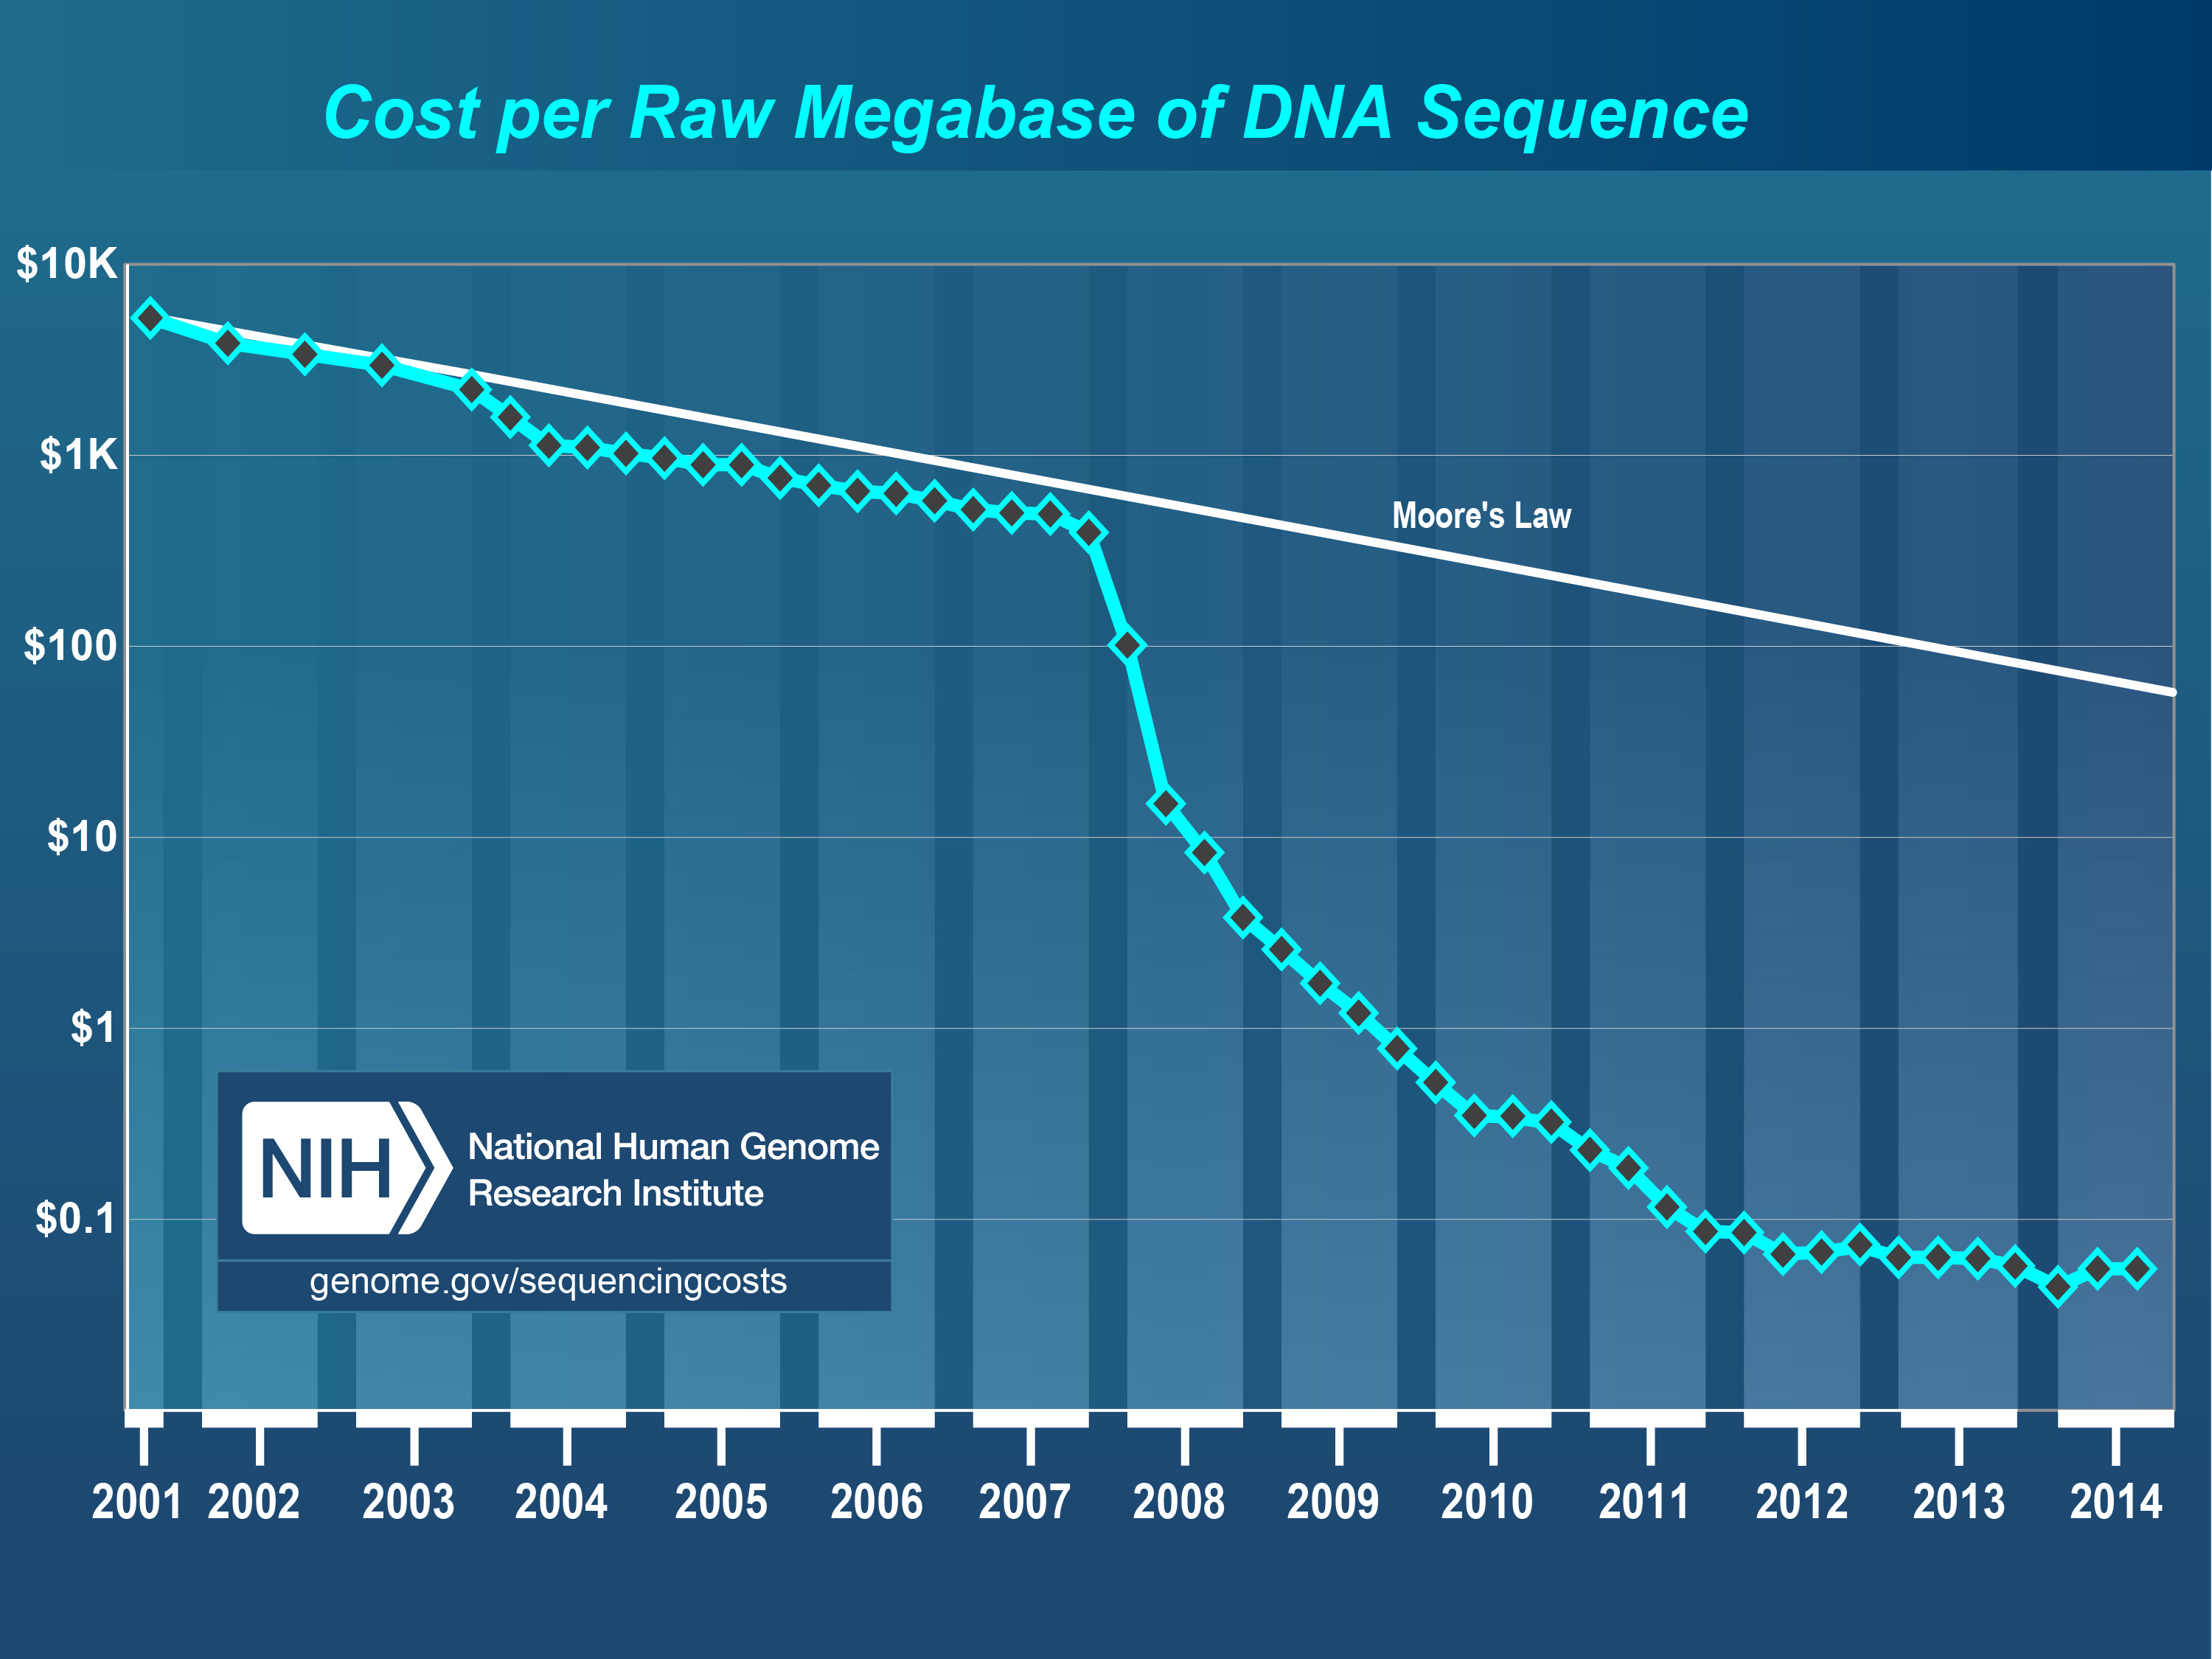
\includegraphics[scale=0.4]{cost_per_megabase.jpg}
  \end{figure}
  \end{center}
\end{frame}

\section{Roche 454 Pyrosequencing}

\begin{frame}
  \frametitle{Roche 454}
  The first massively parallel method to become commercially available was developed by 454 Life Sciences in 2005 (acquired by Roche in 2007) and is based on the pyrosequencing technique. Similar to the Sanger method, sequencing is carried out using primed synthesis by DNA polymerase. However in the 454 pyrosequencing method, the DNA fragments are presented with each of the four dNTPs sequencially and without a dye-terminator, as is done with Sanger sequencing, allowing for multiple incorportation in the same flow. The amount of the incorporation is monitored by luminometric detection of the pyrophosphate released (hence the name "pyrosequencing").
\end{frame}

\begin{frame}
  \frametitle{Roche 454 platforms}
  Roche 454 has 2 platforms the GS Junior System (a "benchtop" system) and the GS FLX+ System (what we have on campus).
  \begin{center}
    \begin{figure}
    \includegraphics[scale=0.4]{Roche_specs.png}
  \end{figure}
  \end{center}
\end{frame}

\begin{frame}
  \frametitle{Roche 454 Workflow}
  \begin{itemize}
  \item Library Construction
  \item QA - Library Quantification (Titration)
  \item emulsion PCR (emPCR)
  \item Picotiter Plate Loading
  \item Sequencing
  \item Image extraction
  \item Flowgram extraction
  \end{itemize}
\end{frame}


\begin{frame}
  \frametitle{Roche 454 Workflow Video}
  \begin{center}
  \href{http://www.youtube.com/watch?feature=player_detailpage&v=bFNjxKHP8Jc}{454 Video}
  \end{center}  
\end{frame}


\begin{frame}
  \frametitle{Roche 454 Flowgrams}
  \begin{center}
    \begin{figure}
    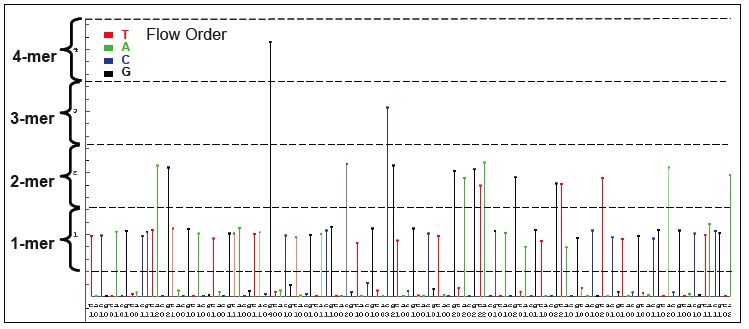
\includegraphics[scale=0.35]{Flowgram.jpg}
  \end{figure}
  \end{center}
\end{frame}

\begin{frame}
  \frametitle{454 Read Naming Convections}
Roche 454 raw data are stored in SFF files (standard flowgram format), but fasta and qual (or fastq) files can be extracted from them\\
  $>$EBO6PME01EGNVK
  \begin{description}
  \item[Timestamp] EB06PM
  \item[Randomized ] E
  \item[Plate Region] 01
  \item[X,Y coord] EGNVK
  \end{description}
  The timestamp, hash character and X,Y location use a base-36 encoding (where values 0-25 are the letters 'A'-'Z' and the values 26-35 are the digits '0'-'9'). An accession thus consists only of letters and digits, and is case-insensitive. 
\end{frame}
   

\section{Illumina/Solexa}

\begin{frame}
  \frametitle{Illumina Solexa}
  The second next-generation sequencing technology to be released (in 2006) was Illumina Solexa sequencing. A key difference between Roche 454 and Illumina sequencing was the use of chain-terminating nucleotides. The fluorescent label on the terminating base can be removed to leave an unblocked 3' terminus, mating the chain termination a reversible process. The method thus sequences one base at a time, rather than 0 or more bases as does Roche 454.
\end{frame}

\begin{frame}
  \frametitle{Illumina Platforms}
Illumina has multiple systems, in three classes\\ MiSeq, NextSeq and HiSeq
    \begin{center}
    \href{http://www.illumina.com/systems.html}{Illumina Systems}
    \end{center}
\end{frame}

\begin{frame}
  \frametitle{Illumina Workflow}
  \begin{itemize}
  \item Library Construction
  \item Cluster Generation
  \item Sequencing
  \item image extraction
  \end{itemize}
\end{frame}


\begin{frame}
  \frametitle{Illumina Workflow Video}
  \begin{center}
  \href{http://www.youtube.com/watch?NR=1&feature=endscreen&v=l99aKKHcxC4}{Illumina Video}
  \end{center}
\end{frame} 

    
\begin{frame}
  \frametitle{Illumina Read Naming Conventions}
  \begin{small}
  @EAS139:136:FC706VJ:2:2104:15343:197393 1:Y:18:ATCACG\\
  \end{small}  
  \begin{description}
  \item[EAS139]	the unique instrument name
  \item[136]	the run id
  \item[FC706VJ]	the flowcell id
  \item[2]	flowcell lane
  \item[2104]	tile number within the flowcell lane
  \item[15343]	'x'-coordinate of the cluster within the tile
  \item[197393]	'y'-coordinate of the cluster within the tile
  \item[1]	the member of a pair, 1 or 2 (paired-end or mate-pair reads only)
  \item[Y]	Y if the read fails filter (read is bad), N otherwise
  \item[18]	0 when none of the control bits are on, otherwise it is an even     number
  \item[ATCACG]	index sequence
  \end{description}
\end{frame}

\section{Life Sciences Ion Torrent}
\begin{frame}
  \frametitle{Ion Torrent Workflow Video}
Ion Torrent PGM, first available in 2011, generates up to 400bp reads (reported) and up to 2Gb (5.5m reads) per run. Cheap fast runs. Ion Proton system can generate up to 10Gb per run. Generates flowgrams and SFF files similar to Roche 454 data as well as the standard fastq files.
  \begin{center}
  \href{https://www.youtube.com/watch?feature=player_embedded&v=MxkYa9XCvBQ}{Ion Torrent Video}
  \end{center}
\end{frame} 

\section {Pacific Biosystems}
\begin{frame}
Pacific Biosystems is so far the most successful third generation DNA sequencing system. Key differences are that its a single molecule, real time (SMRT) technology and capable of producing sequences of multi-kilobases.
  \frametitle{Pacific Biosciences Workflow Video}
  \begin{center}
  \href{http://www.youtube.com/watch?v=NHCJ8PtYCFc&feature=endscreen&NR=1}{Pacific Biosciences Video}
  \end{center}
  \begin{center}
    \begin{figure}
    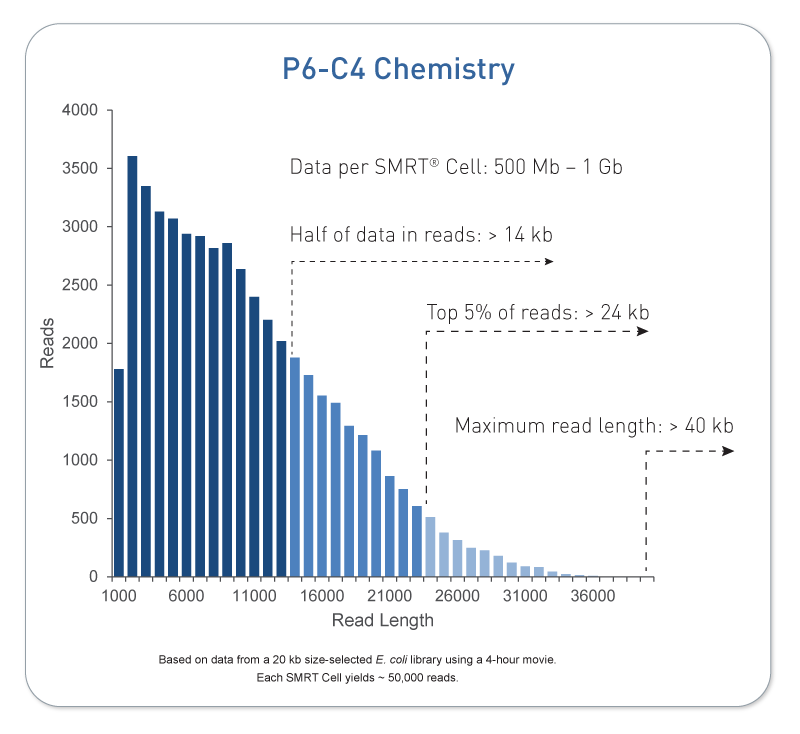
\includegraphics[scale=0.23]{PacBio-specs.png}
  \end{figure}
  \end{center}
\end{frame} 

\section{Oxford Nanopore}
\begin{frame}
Announced in 2012, Oxford Nanopore sent a ripple through the sequencing community but has yet to live up to expectations. Promises "tens of kbs".
  \begin{center}
    \begin{figure}
    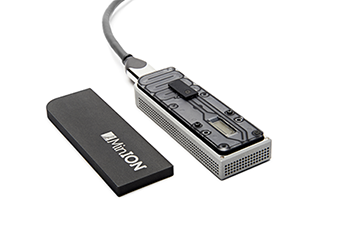
\includegraphics[scale=0.4]{mini_ion_300_open-copy.png}
  \end{figure}
  \end{center}
    \begin{center}
  \href{https://player.vimeo.com/video/77246565}{Minion Video}
  \end{center}

\end{frame}



\end{document}

